\chapter{Bootproces}

\section{Opstarten}

Het opstartproces van een computer begint wanneer de voeding van
de computer ingeschakeld wordt. Bij het inschakelen controleert de
voeding zijn eigen spanningsniveaus. Wanneer de spanning stabiel is
tussen aanvaardbare waarden wordt een 'Power Good'\index{power good} signaal
gestuurd naar het moederbord. Het duurt typisch tussen 0,1 en 0,5
seconden voor de voeding stabiele stroom kan leveren.

Een halve seconde lijkt niet veel, maar de huidige processoren
voeren in die tijd miljoenen instructies uit. Om te vermijden dat het
systeem onder deze onstabiele omstandigheden zou beginnen opstarten
blijft het moederbord de processor continu resetten zolang er geen power
good signaal ontvangen wordt. Ook wanneer de computer al in gebruik is
verhindert dit mechanisme beschadiging of onzekere resultaten door
slechte stroomtoevoer. Bij problemen met de stroomvoorziening, zoals een
abnormale spanningswijziging op het stroomnet, zal het systeem zichzelf
herstarten omdat de processor weer tijdelijk het reset-signaal ontvangt
wanneer het power good signaal vanuit de voeding wegvalt.

Wanneer het reset-signaal wegvalt kan de processor beginnen
werken. De processor draait nu in kernel mode (d.i.: alle instructies 
---ook de gepriviligeerde instructies--- zijn toegelaten) en gebruikt
uit compatibiliteitsoverwegingen \emph{real mode}\index{real mode}
als addresseringsmodus\footnote{Indien je niet meer weet wat \emph{real mode} 
is, dan kan je dat best nog eens opzoeken in hoofdstuk 3 van de cursus
Computersystemen}. Maar welke code moet er uitgevoerd worden? Er zijn nog geen
instructies in het werkgeheugen geladen, dus de opstartcode moet elders
gevonden worden.

De oplossing voor dit probleem is om bepaalde adressen in de geheugenruimte niet
mappen op het werkgeheugen maar op iets anders. Dit noemt men \emph{memory mapped I/O}. Figuur~\ref{memorymapped}
toont de layout van de x86-geheugenruimte en welke stukken waarop gemapped worden.
Het rode stuk in de tekening is het stuk van de geheugenruimte waar de processor
de opstartcode verwacht. Concreet begint de processor instructies uit te voeren 
vanaf adres 0xFFFFFFF0 (merk op dat dit adres binnen het rode stuk valt). Wanneer
de processor het geheugenadres 0xFFFFFFF0 opvraagt aan de geheugen controller, zal
die echter geen bytes vanuit het werkgeheugen halen, maar zal die de data halen uit
een ROM-chip op het moederbord. Deze ROM-chip bevat dan het opstartprogramma.

\begin{figure}
\centering
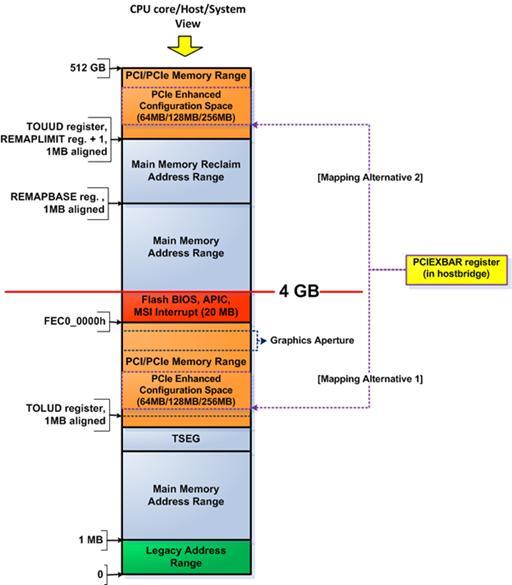
\includegraphics[scale=.75]{images/iomappedmemory.png}
\caption{De x86 memory layout. Leer deze grafiek alsjeblieft niet vanbuiten!}
\label{memorymapped}
\end{figure}

\section{Unified Extensible Firmware Interface}

Moderne systemen volgen de \emph{Unified Extensible Firmware Interface}-specificatie
(\emph{UEFI})\index{UEFI} om de computer verder op te starten. De UEFI-standaard zorgt voor afspraken omtrent een zogenaamde
\emph{pre-boot execution environment} die er voor zorgt dat de hardware ge\"initialiseerd
wordt en het besturingssysteem ingeladen wordt. Implementaties van deze standaard zijn in essentie een
mini-besturingssysteem die een aantal basisfunctionaliteiten aanbieden (zoals bijvoorbeeld
het starten van het hoofdbesturingssysteem).

De belangrijkste eigenschappen die de UEFI-standaard voorziet, zijn:

\begin{itemize}
\item \textbf{Ondersteuning voor grote schijven} De voorganger van UEFI ---{} het Basic Input/Output System (BIOS)\index{basic input/output system} ---{} bood maar ondersteuning voor harde schijven tot 2TB. De UEFI-standaard verhoogt deze limiet tot 8ZB (d.i. 8 miljard terabyte).
\item \textbf{CPU-onafhankelijke architectuur} De UEFI-specificatie is zo opgesteld dat de services die worden aangeboden niet processor-specifiek zijn. Er zijn dan ook UEFI-implementaties voor de x86-, x86-64-, ARM-, ARM64-, en Itanium-processoren.
\item \textbf{CPU-onafhankelijke stuurprogramma's} EFI Byte Code (EBC) is een processor-onafhankelijke machinetaal die een beetje vergelijkbaar is met Java bytecode\footnote{https://en.wikipedia.org/wiki/Java\_bytecode} of Common Intermediate Language\footnote{https://en.wikipedia.org/wiki/Common\_Intermediate\_Language}. Een UEFI-implementatie kan dan een vertolker bevatten om die EBC uit te voeren. Zo moet een auteur van een stuurprogramma slechts \'e\'en versie van het stuurprogramma schrijven (in EBC), dat dan op alle processorarchitecturen waar UEFI op ondersteund wordt kan gebruikt worden.\footnote{In praktijk gaan hardwareontwerpers echter nog vaak processor-specifieke drivers voorzien omdat die vaak een stuk sneller zijn dan de EBC-varianten.}
\item \textbf{Modulair ontwerp} De UEFI-standaard voorziet een aantal mogelijke diensten die kunnen aangeboden worden, maar niet alle diensten \emph{moeten} aangeboden worden.
\item \textbf{Flexibele pre-OS omgeving} Hardwareverkopers krijgen de vrijheid om te kiezen hoe de layout van de pre-OS-omgeving eruit ziet en welke features ze willen ondersteunen. Verder kunnen gebruikers ook nog UEFI-applicaties installeren die dan uitgevoerd worden voordat het besturingssysteem opgestart is. Voorbeelden van zulke applicaties zijn bijvoorbeeld \emph{boot loaders} die dienen om de gebruiker te laten kiezen tussen verschillende besturingssystemen die ge\"installeerd zijn.
\item \textbf{Backward en forward compatibiliteit} UEFI voorziet een compatibiliteits-module om achterwaarts compatibel te zijn met besturingssystemen die geschreven zijn voor de BIOS-voorganger. Verder proberen de auteurs van UEFI ook voorwaarts compatibel te zijn, zodat nieuwe technologie\"en naadloos kunnen gebruikt worden op reeds bestaande UEFI-systemen.
\end{itemize}

UEFI voorziet \emph{boot services} en \emph{runtime services}. Boot services zijn enkel beschikbaar voordat het besturingssysteem opgestart is. Zo zijn er services om uitvoer op het scherm te tonen, communicatie met hardware te verzorgen, enz. De runtime services blijven beschikbaar, ook wanneer het besturingssysteem operationeel is. Zo kan het besturingssysteem bijvoorbeeld de datum en de tijd opvragen, of kan het kleine stukjes data opslaan in de chip waar de UEFI-implementatie in staat.\footnote{Dit is ook de reden waarom je bij het vervangen van een harde schijf je Windows 10 productsleutel niet opnieuw moet ingeven; de Windows 10-setup gaat automatisch je productsleutel opslaan in de UEFI-chip, zodat je die later niet meer opnieuw moet ingeven.}

% \section{Basic Input/Output System (BIOS)}

% Het eerste programma dat de processor uitvoert is het
% \emph{Basic Input/Output System}, vaak afgekort tot
% \emph{BIOS}. Het zorgt dat er communicatie mogelijk is
% tussen enkele onderdelen van het computersysteem, in de eerste plaats
% tussen secundaire opslagapparaten en het werkgeheugen. Zo kunnen
% programma's van b.v. een harde schijf in het werkgeheugen geladen
% worden, en kunnen deze programma's uitgevoerd worden. Het Basic
% Input/Output System dankt zijn naam aan het feit dat het naast deze
% communicatie ook zorgt voor uitvoer op het scherm, en de mogelijkheid
% tot invoer via het toetsenbord. Je kan de BIOS zien als een klein en
% eenvoudig besturingssysteem.

% Aangezien het net de BIOS ervoor moet zorgen dat de
% opslagapparaten bruikbaar worden kan de BIOS-code niet op een dergelijk
% apparaat bewaard worden. Daarom wordt deze code in een ROM-chip op het
% moederbord bewaard. Tegenwoordig wordt EEPROM gebruikt zodat het toch
% mogelijk is een nieuwe versie van de code op de chip te zetten. Deze
% chip wordt ook vaak gewoon 'BIOS' genoemd. Merk op dat de BIOS opnieuw
% een voorbeeld is van firmware.

% Omdat een processor altijd de opdracht uit het werkgeheugen
% inleest waarvan het adres in de bevelenteller staat, wordt de inhoud van
% de BIOS-chip beschikbaar gesteld via een deel van het adresbereik van
% het werkgeheugen. Hiervoor is een deel van het Upper Memory\footnote{De Upper
% Memory Area is de laatste 384 kilobyte van de eerste megabyte van het
% werkgeheugen.} gereserveerd: van F0000h tot FFFFFh. In sommige systemen
% blijft dit deel van het werkgeheugen leeg en wordt van de ROM-chip
% gelezen. Andere systemen kopi\"eren de inhoud van de chip naar dit
% gedeelte van het werkgeheugen omdat RAM sneller is dat ROM. Deze
% techniek wordt \emph{ROM shadowing} genoemd.

% Wanneer een processor geactiveerd wordt zal hij altijd beginnen
% met de instructie op adres FFFF0h\footnote{Het adres FFFF0h wordt ook vaak
% genoteerd als FFFF:0000. De eerste notatie is lineair vanaf de start van het
% werkgeheugen. De tweede notatie geeft aan dat we werken in een geheugensegment
% dat begint op FFFF0, en dat we vanaf dat adres 0 plaatsen verder moeten gaan.}.
% Dit adres ligt in het gebied dat aan de BIOS is toegekend, maar ligt achteraan.
% Hier staat dan een JMP (jump) instrucie naar de eigenlijke opstartcode.

\begin{figure}
\centering
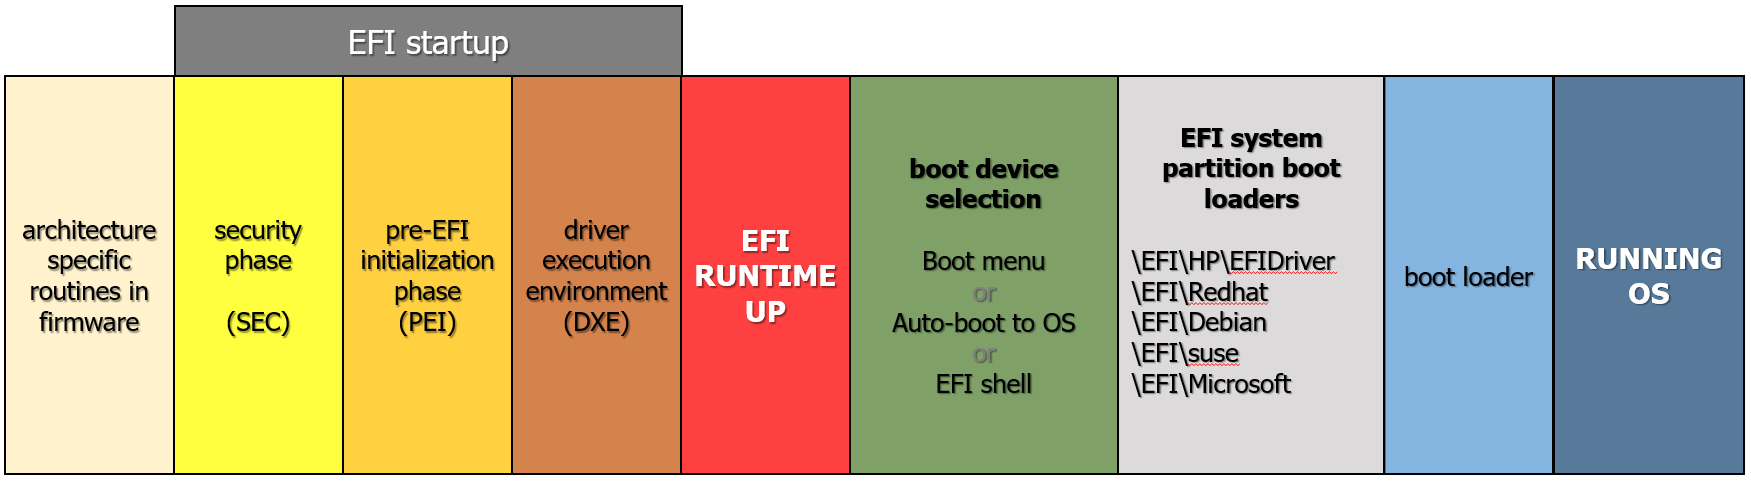
\includegraphics[scale=.25]{images/uefisartup.png}
\caption{Het UEFI boot-proces}
\label{uefiboot}
\end{figure}

De UEFI-specificatie voorziet een aantal fases tijdens het opstarten, zoals weergegeven in Figuur~\ref{uefiboot}.
In de eerste fases gaat het systeem de EFI-runtime opstarten. Binnen deze runtime kunnen dan allerhande
UEFI-applicaties uitgevoerd worden.

De UEFI-specificatie bepaalt niet hoe de machine opgestart moet worden. Typisch zullen UEFI-implementaties beginnen met
het oplijsten van alle beschikbare stukken hardware en controleren of die correct werken. Het geheel van deze tests
wordt \emph{Power-On Self Test}\index{power-on self test} genoemd, of kortweg \emph{POST}. Op sommige systemen kan je kiezen om deze POST
aan te passen of grotendeels over te slaan. Het voordeel is dan dat je computer sneller opstart, maar je zal een aantal
opties (zoals het opstarten vanaf een USB stick) niet meer kunnen gebruiken.

% De BIOS-opstartcode begint met het testen van de vitale
% systeemonderdelen. Het geheel van deze tests wordt \emph{Power-On
% Self Test} genoemd, of kortweg \emph{POST}.
% De aanwezigheid en/of correcte werking van b.v. de processor,
% werkgeheugen en toetsenbord worden getest. De feedback gebeurt d.m.v.
% geluidssignalen die we beeps noemen. Wanneer alles naar behoren werkt
% wordt meestal 1 korte beep weergegeven. Bij problemen kan men aan het
% aantal beeps en hun duur horen wat de oorzaak is. De concrete codes
% hangen af van de producent van de BIOS. Soms wordt bijkomend gebruik
% gemaakt van bijkomende indicaties van problemen, zoals een digitaal
% display of LEDs.

Als de initialisatie succesvol voltooid is zal de UEFI-code beginnen met
het laden van het besturingssysteem. Dit staat typisch op een
secundair opslagapparaat. Wanneer een computersysteem meerdere van
dergelijke opslagapparaten bevat moet de gebruiker aangeven vanop
welk apparaat een besturingssysteem geladen moet worden. Het
besturingssysteem kan op een harde schijf staan, maar het zou ook op
een CD-ROM, diskette of USB-opslagapparaat. In welke volgorde op alle
aanwezige apparaten naar een besturingssysteem gezocht moet worden
staat in de zogenaamde \emph{opstartvolgorde} of
\emph{boot sequence}\index{boot sequence}. De gebruiker kan deze opstartvolgorde naar eigen keuze aanpassen.

% Naast de opstartvolgorde kan je
% mogelijk ook instellingen voor bepaalde randapparaten of een paswoord
% dat de instellingen wijzigen.

% Omdat deze instellingen gewijzigd moeten kunnen worden kunnen ze
% niet samen met de code van de BIOS bewaard worden in een ROM-chip.
% Voor de veranderlijke BIOS-instellingen is een afzonderlijke CMOS-chip
% voorzien, die door een batterij onder spanning gehouden wordt wanneer
% het systeem uitgeschakeld is. Zo gaan de instellingen niet verloren.
% Omdat het in het begin de enige component met CMOS-technologie was
% wordt de chip met de BIOS-instellingen nog vaak 'CMOS' genoemd. In
% hedendaagse computersystemen worden echter ook de processoren en het
% werkgeheugen m.b.v. CMOS ge\"implementeerd.

\section{Schijven en partities}

% TODO: EFI System Partition

%\begin{figure}
%\begin{center}
%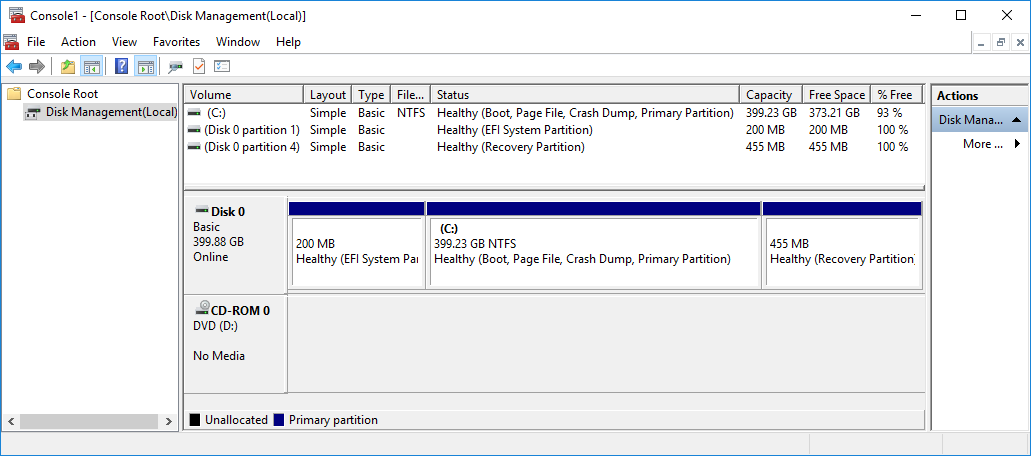
\includegraphics[width=125mm]{images/diskmgr.png}
%\end{center}
%\caption{DE EFI System Partition}
%\label{efisyspart}
%\end{figure}

% https://msdn.microsoft.com/en-us/library/windows/desktop/aa365449(v=vs.85).aspx


Als in de opstartvolgorde verwezen wordt naar een harde schijf
is de vraag weer hoe we het besturingssysteem terugvinden. De schijf kan in verschillende stukken
opgedeeld zijn (zogenaamde \emph{partities})\index{partitie}, en op eender welke partitie kan het besturingssysteem staan.
Het is aan de gebruiker om via de UEFI-gebruikersinterface de juiste partitie te kiezen.

Het opsplitsen van een schijf in verschillende stukken heeft praktisch nut:
\begin{itemize}
\item Er kan een partitie worden gemaakt voor de bestanden van het besturingssysteem, die enkel bestaat uit de snelste sporen van de schijf.\footnote{\textbf{vraag:} \emph{Welke sporen op de harde schijf zijn de snelste? Denk aan de `zone bit recording'-technologie die in Computersystemen besproken is.}}
\item Het systeem is iets robuuster: je kan makkelijker de beveiliging per partitie instellen, als een programma vanwege een bug de schijf helemaal vult dan heb je daar maar last van op \'e\'en partitie, ...
\item Verschillende partities kunnen verschillende besturingssystemen bevatten (dit noemt men een zogenaamde \emph{multiboot}-opstelling)\index{multiboot}.
\item Zorgt voor een duidelijk scheiding tussen bijvoorbeeld het systeem en databestanden.
\item ...
\end{itemize}

Indien de gebruiker op meerdere partities een besturingssysteem ge\"installeerd heeft, dan kan er een
\emph{boot manager}\index{boot manager} gebruikt worden. De boot manager toont tijdens het opstartproces een lijst van alle
ge\"installeerde besturingssystemen en laat de gebruiker kiezen welke hij wil opstarten. Figuur~\ref{fig:bootloaders}
toont twee voorbeelden van boot managers.

\begin{figure}
\centering
\begin{subfigure}{.5\textwidth}
  \centering
  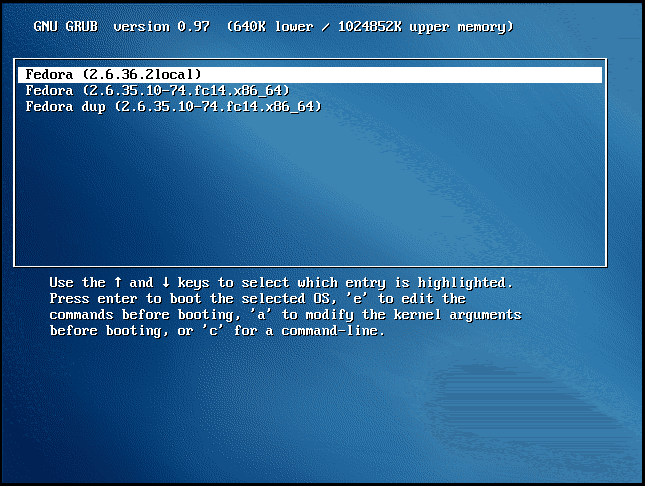
\includegraphics[width=.95\linewidth]{images/grubbl.png}
  \caption{De GRUB boot manager}
  \label{fig:grubnl}
\end{subfigure}%
\begin{subfigure}{.5\textwidth}
  \centering
  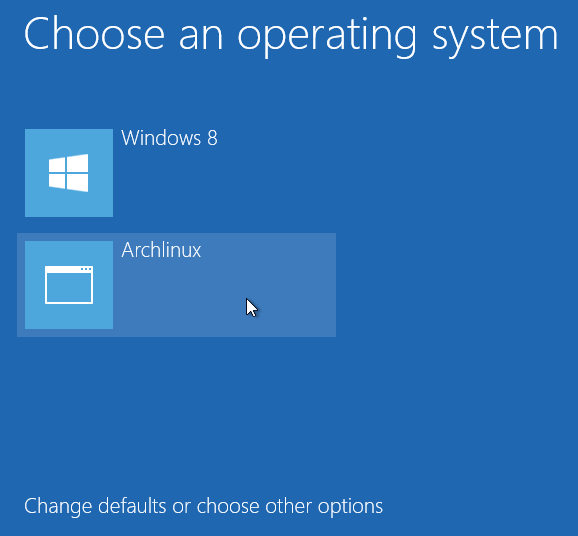
\includegraphics[width=.95\linewidth]{images/wbl.png}
  \caption{De Windows boot manager}
  \label{fig:wbl}
\end{subfigure}
\caption{Twee verschillende UEFI boot managers}
\label{fig:bootloaders}
\end{figure}

Informatie over de partities wordt op de schijf zelf opgeslagen op een gestandardiseerde manier. UEFI ondersteunt de oudere \emph{master boot record}-manier\index{master boot record} (MBR) om partitie-informatie op te slaan, maar deze manier biedt maar ondersteuning voor schijven tot 2TB. Bij voorkeur wordt dan ook het nieuwere \emph{GUID partition table}-systeem\index{GUID partition table} (GPT) gebruikt. GPT biedt ondersteuning voor schijven tot 8ZB (d.i. 8 miljard TB).

Figuur~\ref{fig:gpt-layout} toont de layout van een GPT-schijf. Het eerste blok bevat een \emph{protective master boot record}\index{protective master boot record} voor compatibiliteitsdoeleinden met oudere systemen die geen GPT ondersteunen. Deze protective master boot record is grotendeels leeg, en bevat slechts informatie over \'e\'en partitie die de hele schijf beslaat (of voor schijven groter dan 2TB: zo veel plaats beslaat als mogelijk). Het partitietype staat op \byte{EE} wat betekent dat de partitie in feite een GPT-partitie is. Tools die GPT niet ondersteunen zullen dit partitietype niet herkennen, en zouden normaal gezien de partitie (en dus de schijf) met rust laten.

\begin{figure}
\centering
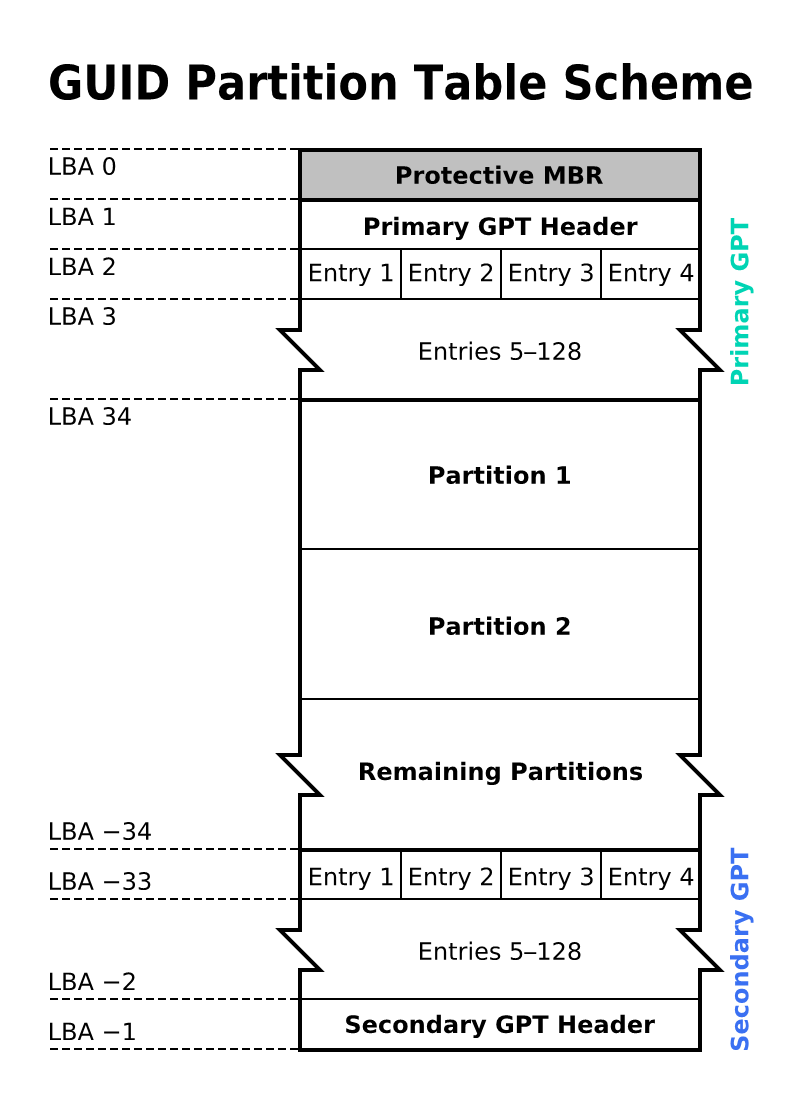
\includegraphics[scale=1]{images/gpt-layout.png}
\caption{De layout van een GPT-schijf}\label{fig:gpt-layout}
\end{figure}

Na de protective MBR staat de primaire GPT header. Deze header bevat informatie over de schijf (grootte, beschikbare sectors, ), een uniek identificatienummer van de schijf, en een wijzer naar een backup-kopie van de header. Deze backup-kopie staat helemaal aan het eind van de schijf en bevat exact dezelfde informatie. Als de primaire header beschadigd raakt, dan kan de backupkopie gebruikt worden om alsnog de partitie-informatie uit te lezen.

Na de primaire GPT header volgt een lijst van \emph{partition entries}.\index{partition entry} Elk van deze entries kan informatie bevatten over \'e\'en partitie. Zo bevat een entry onder andere informatie over het partitietype, een uniek identificatienummer, de start- en eindsector, en de attributen van de partitie (alleen-lezen, verborgen, ...). Ook van de lijst van partition entries wordt een backup op het einde van de schijf bijgehouden.


% De code in de UEFI-implementatie zal een sprong uitvoeren naar opstartcode die
% opgeslagen is op de eerste sector van de schijf, de \emph{Master
% Boot Record} (\emph{MBR}). Deze code wordt
% vaak Initial Program Loader (IPL) genoemd. Na het uitvoeren van de
%BIOS-code zal de processor dus verdergaan met deze code uit de
%MBR.

%Een harde schijf kan logisch ingedeeld worden in
%\emph{partities}. Hierdoor kunnen we meerdere
%besturingssystemen op \'e\'en schijf bewaren, of kunnen we op \'e\'en schijf
%verschillende bestandssystemen gebruiken (zie verder).

%In de \emph{partitietabel} wordt het begin- en
%eindpunt en het type van iedere partitie opgeslagen. Op het
%PC-platform vind je de partitietabel in de MBR, achter de opstartcode.
%De opstartcode neemt 446 bytes in beslag. Er is dan nog plaats voor 4
%maal een partitiebeschrijving van 16 bytes, en een 'magic number' van
%2 bytes. Dit magic number is een controlgetal, en het moet de waarde
%0xAA55 bevatten, anders beschouwt de BIOS de MBR als ongeldig.

%\begin{figure}
%\begin{center}
%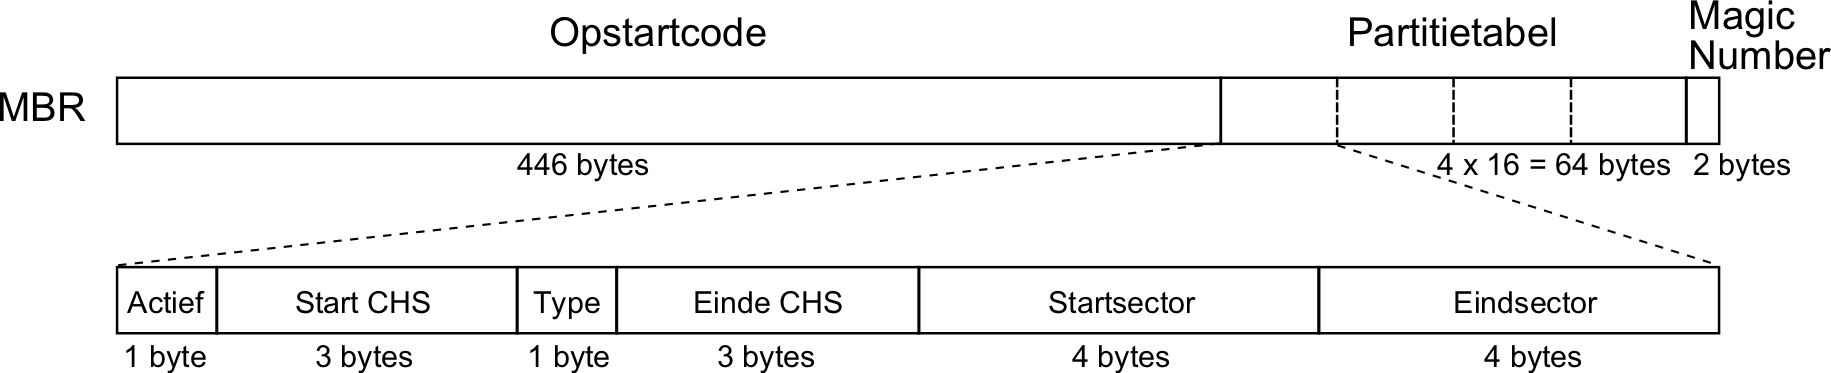
\includegraphics[width=125mm]{images/fig0206.png}
%\end{center}
%\caption{Master Boot Record}
%\label{mbr}
%\end{figure}

%Elk van de 4 elementen van de partitietabel beschrijft een
%partitie, en bevat de volgende velden:

%\begin{description}
%\item[Active] geeft aan of deze partitie opgestart moet worden
%\item[Start] Cylinder / Kop / Sector adres van de eerste sector van de partitie
%\item[Type] Indicatie van het gebruikte bestandssysteem op de partitie
%\item[End] Cylinder / Kop / Sector adres van de laatste sector van de partitie
%\item[Startsector] LBA-adres van de eerste sector van de partitie
%\item[Lengte] Lengte van de partitie
%\end{description}

%De volledige structuur van de MBR en de partitietabel vind je in figuur
%\ref{mbr}.

%De partities die in de partitietabel gedefinieerd worden noemen
%we \emph{primaire partities}. Doordat schijven steeds
%groter werden, was 4 partities voor \'e\'en schijf niet meer genoeg. Om
%meer partitities toe te laten, introduceerde men \emph{logische
%partities}. Er is geen plaats om de partitietabel uit te
%breiden, dus wordt een primaire partitie onderverdeeld in logische
%partities. Een primaire partitie die verder onderverdeeld wordt noemen
%we een '\emph{extended partitie}'. Deze oplossing is
%\emph{achterwaarts compatibel}. Een ouder systeem dat
%niets afweet van het bestaan van extended partities kan de gewone
%primaire partities nog steeds gebruiken.

%In de partitietabel geven de types 0x05 of 0x0f een extended
%partitie aan. Het start-veld bevat dan het adres van de eerste sector
%van de eerste logische partitie. Iedere logische partitie verwijst
%naar de volgende logische partitie. Zo is er geen beperking van het
%aantal logische partities door de grootte van de gebruikte tabel. Een
%structuur waarin ieder element verwijst naar het volgende noemen we
%een \emph{gelinkte lijst}. Als limiet voor het aantal
%logische partities wordt vaak 24 opgegeven. De gelinkte lijst kan
%zonder problemen langer zijn, maar aangezien MS-DOS letters vanaf 'C'
%toekent aan partities kunnen er niet meer dan 24 partities
%zijn\footnote{Opgelet, als je 2 primaire partities en 1 extended partitie
%cre\"eert, kan je in de extended partitie natuurlijk nog maar 22 logische
%partities aanmaken als je wil dat MS-DOS ze allemaal kan bereiken.}.

%Een logische partitie bevat een \emph{Extended
%MBR} (\emph{EMBR}), met een eigen
%partitietabel. Zo'n EMBR bevat een partitietabel die de structuur van
%de tabel in de MBR volgt, maar slechts twee partities beschrijft: \'e\'en
%logische en een nieuwe extended partitie. Deze extended partitie bevat
%ook weer zo'n tabel die \'e\'en logische en \'e\'en extended partitie
%beschrijft, enz.

De taak van de opstartcode is om in de
partitietabel de gewenste opstartpartitie op te sporen. De eerste sector van
deze partitie heet de \emph{partition boot sector} of wordt soms ook de
\emph{partition boot block} of het \emph{partition boot record} genoemd.\index{boot sector} Deze boot sector
bevat ook weer een stuk opstartcode. De code in de UEFI-implementatie zal de bootsector van
de gewenste GPT-partitie in het geheugen zetten, en die dan uitvoeren door er naar te springen. Het is de code in
de boot sector die uiteindelijk het besturingssysteem op de partitie zal inladen en
starten. Deze code wordt in de boot sector geplaatst tijdens
de installatie van het besturingssysteem en verschilt dus ook van besturingssysteem tot besturingssysteem. In het geval van Windows zal de code in de boot sector het programma \emph{bootmgr} in het geheugen laden en opstarten. In het
geval dat dit bestand niet gevonden wordt, zal er een foutmelding op het scherm getoond worden.
Bootmgr is dan de laatste schakel in het bootproces. Dit programma gaat de feitelijke code van Windows inladen en opstarten.
